\documentclass[crop,tikz,10pt]{standalone}

\usepackage{tikz-qtree}
\usetikzlibrary{positioning}

\definecolor{bg1}{RGB}{244,231,195}
\definecolor{bg2}{RGB}{234,204,161}
\definecolor{l1}{RGB}{209,148,106}

\begin{document}

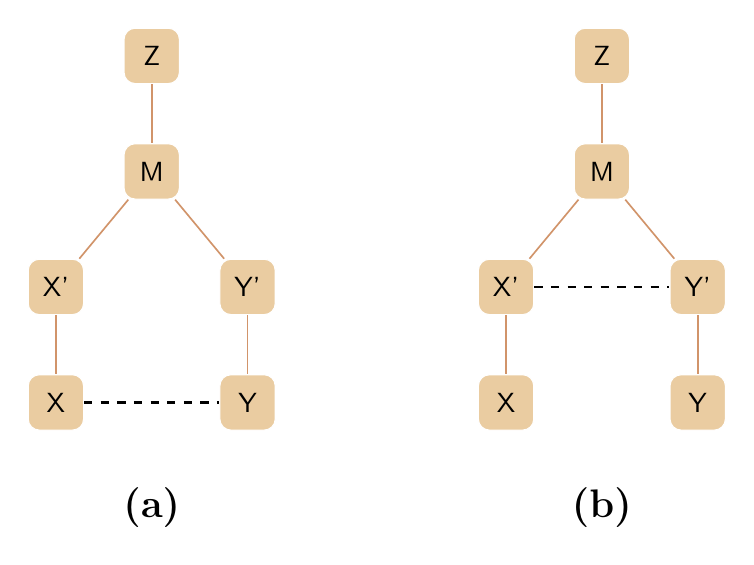
\begin{tikzpicture}[
    font=\sffamily,
    l/.style={
        line width=0.6pt,
        color=l1
    },
    e/.style={
        rounded corners, minimum size=2em,
        fill=bg2, draw=white, line width=0.4pt
    },
    d/.style={dashed, line width=0.8pt},
    label/.style={font=\rmfamily\Large\bfseries}
]

\node [e] (Z) {Z};
\node [e,below=0.75cm of Z] (M) {M};
\node [e,below left =0.75cm and 0.5cm of M] (X') {X'};
\node [e,below right=0.75cm and 0.5cm of M] (Y') {Y'};
\node [e,below=0.75cm of X'] (X) {X};
\node [e,below=0.75cm of Y'] (Y) {Y};

\draw (Z) edge [l] (M);
\draw (M) edge [l] (X');
\draw (M) edge [l] (Y');
\draw (X') edge [l] (X);
\draw (Y') edge [l] (Y);

\draw [d] (X) edge (Y);

\node [label, below=5cm of Z] {(a)};



\node [e, right=5cm of Z] (Z) {Z};

\node [e,below=0.75cm of Z] (M) {M};
\node [e,below left =0.75cm and 0.5cm of M] (X') {X'};
\node [e,below right=0.75cm and 0.5cm of M] (Y') {Y'};
\node [e,below=0.75cm of X'] (X) {X};
\node [e,below=0.75cm of Y'] (Y) {Y};

\draw (Z) edge [l] (M);
\draw (M) edge [l] (X');
\draw (M) edge [l] (Y');
\draw (X') edge [l] (X);
\draw (Y') edge [l] (Y);

\draw [d] (X') edge (Y');

\node [label, below=5cm of Z] {(b)};

\end{tikzpicture}

\end{document}
